\chapter{Wiadukt WK2 w ciągu Pomorskiej Kolei Metropolitalnej}
\section{Budowa modelu numerycznego}
\section{Badania - identyfikacja modalna: wybór punktów, opis badań, wyniki identyfikacji}
Zastosowane kryteria: max mac 0.6, rowno na obie strony, maksymalna srednia z wektorow punktow. Dodac zmiennosc w kombinacjach maksymalnego momentu jako przestroge.
\begin{figure}[h]
	\centering
	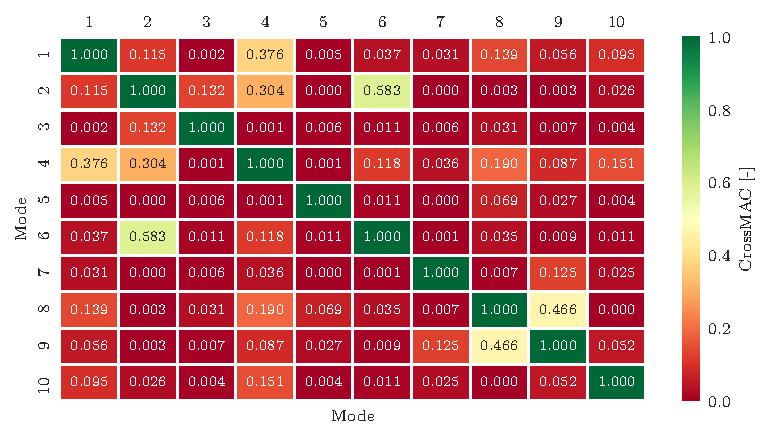
\includegraphics[width=\textwidth]{correlogram_badania.pdf}
	\captionsetup{justification=centering}
	\caption{Diagram AUTOMAC dla pierwszych dziesięciu wektorów postaci drgań własnych, odczytanych z modelu dla wybranych punktów pomiarowych}
\end{figure}
\begin{figure}[h]
	\centering
	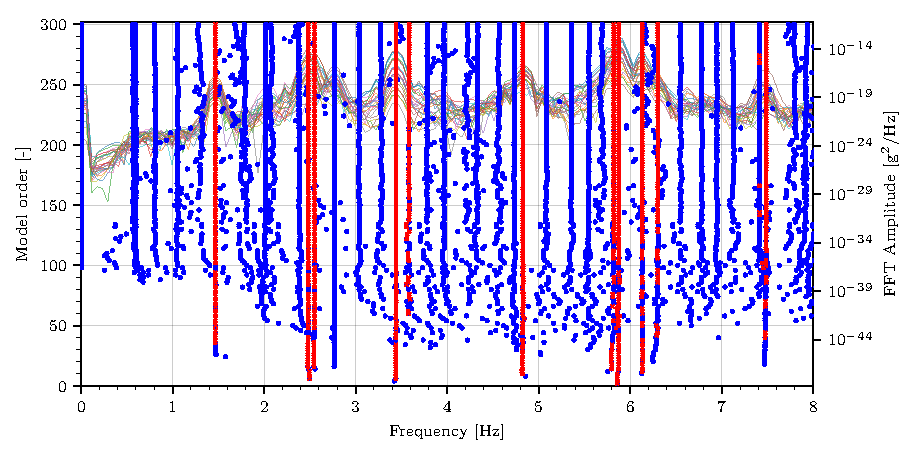
\includegraphics[width=\textwidth]{diagram_non_filtered.pdf}
	\captionsetup{justification=centering}
	\caption{Diagram stabilizacyjny metody NExT-ERA.}
\end{figure}
\begin{figure}[h]
	\centering
	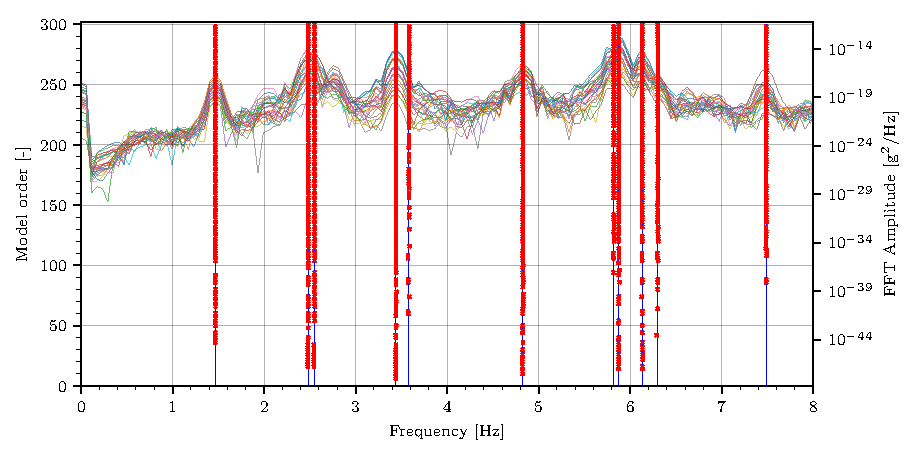
\includegraphics[]{diagram_filtered2.pdf}
	\captionsetup{justification=centering}
	\caption{Diagram stabilizacyjny metody NExT-ERA.}
\end{figure}
\begin{figure}[h]
	\centering
	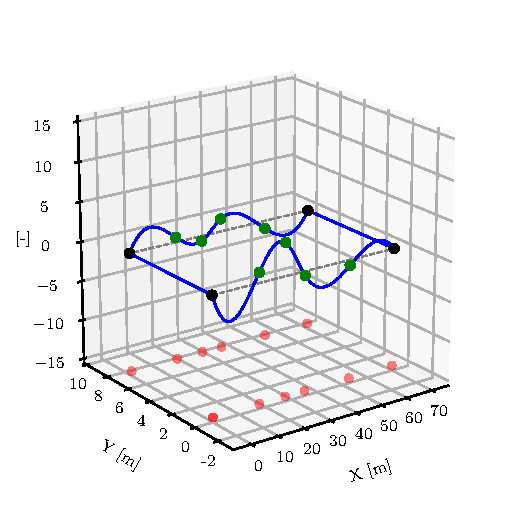
\includegraphics[]{identified_mode_1.pdf}
	\captionsetup{justification=centering}
	\caption{Diagram stabilizacyjny metody NExT-ERA.}
\end{figure}

\section{Kalibracja modelu numerycznego z wykorzystaniem PSO}
\section{Wielokryterialna optymalizacja modelu: opis + wyniki}
\chapter{Podsumowanie i wnioski}
Podsumowania wnioski